\chapter{Introduction}

Reference documentation is widely used in software development to document project APIs, making the development process much easier.
It provides an overview of the types and members declared in the project, along with their documentation comments.
Reference documentation is typically generated by a program called a reference documentation generator (or simply a documentation generator).
Some programming languages include a standard reference documentation generator as part of their SDK (such as \texttt{Javadoc} for Java). 
In other languages, there's a well-established third-party generator, e.g. \texttt{Sphinx} for Python.
However, in .NET, the situation is quite different.
There are multiple generators available, including \texttt{DocFX}, \texttt{Doxygen}, and \texttt{SHFB}, each having its own advantages and limitations.
This brings us to the primary goal of the thesis -- to develop a reference documentation generator for .NET.

\section{Reference documentation use cases}

Before moving on the goals of the thesis, it's important to describe the use cases of reference documentation.
The reference documentation is primarily used by two groups of people:

\begin{itemize}
    \item \textbf{Developers using the library} access the reference documentation to view the library's documented API. 
    Typically, only publicly visible types and members are included. 
    Users typically reach the reference documentation via links from the user documentation.
    \item \textbf{Developers maintaining the library} may also use the reference documentation, although this use case is slightly less common.
    Here, the primary goal of the documentation is to help the programmers understand the internal structure of the project. 
    It is very beneficial during the process of onboarding new team members. 
    In this case, the documentation often includes non-public members as well.
\end{itemize}

The reference documentation may be created in many formats, such as HTML, Markdown, or LaTeX, with HTML being the most common.

Figure~\ref{fig:ref-doc-example} shows an example reference documentation for the \texttt{User} class generated by \texttt{Doxygen}.
Notice that there's a dedicated page for the type containing its documentation \textit{(A)} as well as the list of the declared members with the corresponding documentation comments \textit{(B)}. 
There is also a menu with the search bar at the top of the page \textit{(C)}.
The same observations apply to the vast majority of reference documentation pages, regardless of the generator.

No matter the intended usage, the following features of the resulting documentation are usually required by users.
\begin{enumerate}
    \item Modern UI
    \item Support for cross-references (e.g. a method returning type \texttt{X} should contain a link to its definition if it's declared in the same project)
    \item Search bar
\end{enumerate}

Zero Configuration Build

Support for custom templates

Multiplatform

Documentation versioning

Support for .NET languages

These 3 features also may be presented as goals of our program.
Since we want to support both user scenarios outlined above, we also need to include an option to select private/public members.

(TODO: nejake shrnuti?)

\begin{figure}
\centering
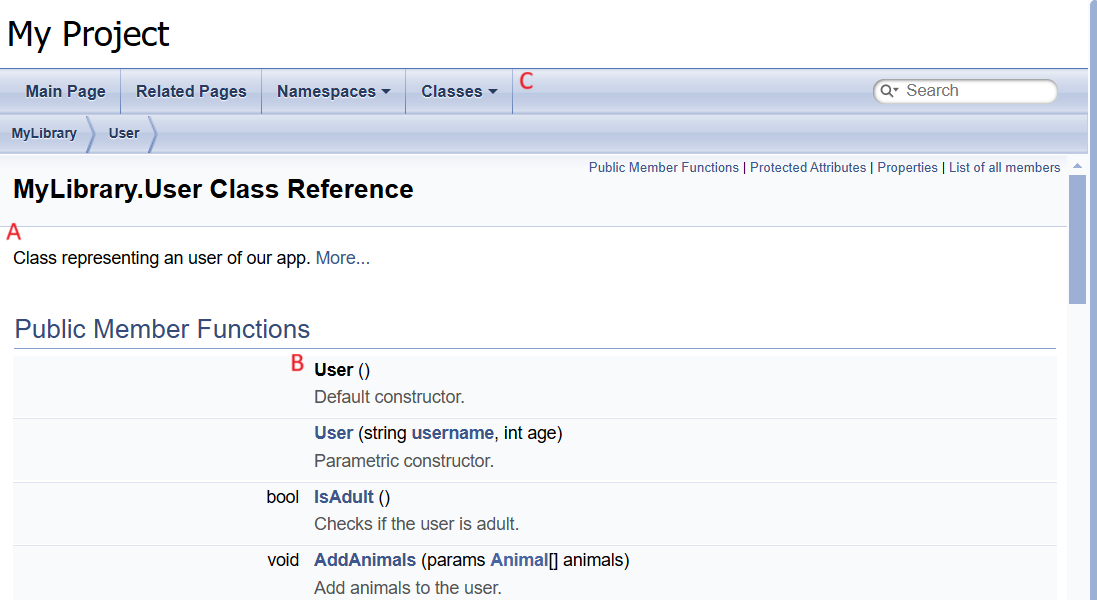
\includegraphics[width=1\linewidth]{img/ref-doc-example.png}
\caption{Reference documentation generated by Doxygen}
\label{fig:ref-doc-example}
\end{figure}

\section{SSGs}

Reference documentation is often accompanied by user documentation, which typically consists of text and code snippets.

We can write user documentation in HTML; however, there's a much easier way to do it -- using a static site generator (SSG).
SSGs, such as Jekyll or MkDocs, are programs 
that use text written in a markup language (often Markdown) to create static web pages.

SSGs enable us to focus only on the textual content of the documentation, and no HTML or CSS knowledge is  required, which is a great advantage.
When building the documentation, we typically just select one of the provided HTML templates to create the webpage.

Many reference documentation generators, for instance, DocFX have at least some of the capabilities of SSGs. 
However, it is possible to use 
the reference documentation generator solely for the reference docs and
create the user documentation using SSG.

(TODO: zminit i nejakou zakladni podporu pro static straneky naseho generatoru?)
